\chapter{Umsetzung der Use-Cases und Evaluation} \label{Umsetzung der Use-Cases und Evaluation}

\section{Use-Case 1: Basis Deployment} \label{Use-Case 1: Basis Deployment}
%IPAM-Vorbereitungen, TF Matching erläutern
%Was ist ein Subnet im Cloud-Kontext? Einleitung?
%TF: Resource, Data, Modul, Provider
\subsection{Umsetzung: Kerntätigkeiten}

Im PHPIPAM müssen mehrere Netzbereiche reserviert werden. Es werden Netzbereiche benötigt, in denen Maschinen per IPv4 kommunizieren können. Diese Netze werden mit VPC bzw. VNET assoziiert. Für VNET wurde der Netzblock \glqq 10.32.0.0/16\grqq{} und für VPC der Netzblock \glqq 10.33.0.0/16\grqq{} vorreserviert, aus dem kleinere Subnets für die jeweilige Cloud entnommen werden können. Weiterhin ist die Annahme, dass die Private Cloud bereits einen Netzbereich besitzt, in dem Maschinen angesiedelt sind: \glqq 192.168.201.0/24.\grqq{}\\
%https://docs.aws.amazon.com/vpn/latest/s2svpn/VPNTunnels.html
%https://docs.microsoft.com/de-de/azure/vpn-gateway/bgp-howto
Weiterhin benötigt man {Transfernetzwerke}, über die die IPv4-Pakete geschickt werden und die BGP-Präfixe ausgetauscht werden können. AWS sieht hierfür /30-Präfixe aus dem Bereich \glqq 169.254.0.0/16\grqq{} vor, Azure hat eine Range reserviert: \glqq 169.254.21.0 - 169.254.22.255\grqq{}. Als Kompromiss können daher nur Netze aus den Azure-Bereichen genutzt werden, da die Bereiche, die AWS zur Verfügung stellt, größtenteils außerhalb dieser Range liegen. Auch diese Netzbereiche müssen im IPAM vorreserviert werden, auch die Transfernetze automatisiert ausgebracht werden.\\
Im folgenden Code-Beispiel wird innerhalb des IPAM nach dem Bereich \glqq TF\_CLOUD\_BGP\_TRANSFER\grqq{}, aus dem alle Transfernetze entommen werden, gesucht. Innerhalb des Bereichs wird aus dem vorreservierten Block \glqq Cloud\_Transfer\_BGP\_1\grqq{} ein /30-Netzwerk entnommen. Die Reservierung der Netzblöcke für VPC und VNET erfolgen analog.
%data vs. resource in Einleitung erläutern?
\FloatBarrier
\begin{lstlisting}[float,label=network-reservation-ip,caption=Die data-Anweisungen dienen ausschließlich der Suche nach dem passenden Transfernetzwerk-Block. Per resource-Anweisung wird ein /30-Netzwerk reserviert.]
//Azure - AWS Transfer
data "phpipam_section" "apipa_main_section" {
  name = "TF_CLOUD_BGP_TRANSFER"
}
data "phpipam_subnet" "apipa_transfer_subnet" {
  section_id = data.phpipam_section.apipa_main_section.section_id
  description_match = "Cloud_Transfer_BGP_1"
} 
resource "phpipam_first_free_subnet" "free_subnet_apipa" {
  parent_subnet_id = data.phpipam_subnet.apipa_transfer_subnet.subnet_id
  subnet_mask = 30
  description = "BGP_AWS_AZURE"
}
\end{lstlisting}
\FloatBarrier
Es ist auch möglich, dass IPv4-Adressen für Transfernetze automatisch von Azure bzw. AWS vorgegeben werden. Mit dem avisierten Backbone-Design aus drei Teilnehmern lässt sich das allerdings nicht vereinbaren: die Adressbereiche müssen vom IPAM vorgegeben werden (vgl. später: Probleme statische Route).\\
Weiterhin werden Pre-Shared-Keys für die Aushandlung der IPSEC-Verbindungen benötigt. AWS erzeugt automatisch solche Schlüssel, welche durch das Terraform-Modul \glqq aws\_vpn\_connection\grqq{} zurückgegeben werden. Diese automatisch erzeugten Schlüssel werden daher für die Backbone-Verbindungen AWS <-> Azure und AWS <-> Private Cloud (VyOS) genutzt. Da Azure diese Schlüssel nicht erzeugt, wurde ein Terraform-Modul geschrieben, welches diese Schlüssel aus 24 Zeichen erzeugt. Dieses kann anschließend genutzt werden für die Backbone-Verbindung Azure <-> Private Cloud (VyOS).

\begin{lstlisting}[label=tf-generate-psk,caption=Auf Sonderzeichen (special) wurde verzichtet. Das Modul stellt per output-Anweisung den Schlüssel für andere Terraform-Module zur Verfügung.]
resource "random_password" "random_password" {
  length = 24
  lower = true
  upper = true
  number = true
  special = false
}
output "azure_vyos_tunnel1_psk" {
  value = random_password.random_password.result
  sensitive = true
}
\end{lstlisting}

%alles Devices nennen?
Da, wie bereits erwähnt (vgl. klick), für die VyOS-Router keine Terraform-Integration verfügbar ist, wurde zur Konfiguration des Devices eine Vorlage erstellt.

%https://www.terraform.io/docs/language/functions/templatefile.html
Die Erzeugung der Vorlage erfolgt über die Funktion templatefile().

\begin{lstlisting}[label=tf-call-tpl-generation,caption=Die Funktion templatefile() erzeugt aus einer Template-Datei (vyos\_config.tpl) die Datei /tmp/example.sh. Die Template-Datei wird mit den Variablen var.aws\_vgw\_ip und aws\_tunnel1\_psk befüllt.]
resource "local_file" "vyos_config" {
  filename = /tmp/example.sh
  content = templatefile("${path.module}/include/vyos_config.tpl",
  {
    aws_vgw_ip = var.aws_vgw_ip
    aws_tunnel1_psk = var.aws_tunnel1_psk
    [ ... weitere Aufrufparameter ...]
  })
}
\end{lstlisting}

\begin{lstlisting}[label=tf-generate-tpl,caption=Verschiede set-Kommandos werden in ein VyOS-Skript eingebettet (Interpreter: /bin/vbash). Die Variablen in Zeilen 9-12 resultieren aus dem Funktionsaufruf (s.o.).]
$ head -n 11 < vyos/include/vyos_config.tpl
#!/bin/vbash
source /opt/vyatta/etc/functions/script-template
configure
#AWS
set vpn ipsec ike-group AWS lifetime '28800'
set vpn ipsec ike-group AWS proposal 1 dh-group '2'
set vpn ipsec ike-group AWS proposal 1 encryption 'aes128'
set vpn ipsec ike-group AWS proposal 1 hash 'sha1'
set vpn ipsec site-to-site peer ${aws_vgw_ip} authentication mode 'pre-shared-secret'
set vpn ipsec site-to-site peer ${aws_vgw_ip} authentication pre-shared-secret ${aws_tunnel1_psk}
set vpn ipsec site-to-site peer ${aws_vgw_ip} description 'VPC tunnel 1'
\end{lstlisting}

\begin{lstlisting}[label=tf-generate-psk,caption=Das so generierte Shell-Skript wird per SSH auf das Zielsystem (VyOS-Router) hochgeladen und per provisioner remote-exec ausgeführt.]
resource "null_resource" "vyos_config" {
  connection {
    type = "ssh"
    host = var.vyos_host
    user = var.ssh_user
    private_key = file(var.private_key_file)
  }
  provisioner "file" {
   source = /tmp/example.sh
   destination = var.vyos_script_path
  }
  provisioner "remote-exec" {
    inline = [ "chmod +x ${var.vyos_script_path}", var.vyos_script_path ]
  }
}
\end{lstlisting}

\newpage
\subsection{Probleme und Lösungsfindung}
%Probleme: Race Condition externe IP, Redeploy wegen TF Bug, statische Route zu BGP Neighbor (Azure - AWS: Pseudo directly, Azure - VyOS: Static, Azure - AWS), stateless VyOS Config, lange Laufzeiten Erstellung VPN Gateway Azure

\textbf{\underline{Vertauschung von IPSEC-Tunnelparametern}}

%https://github.com/hashicorp/terraform-provider-aws/issues/396
AWS VPN-Verbindungen bieten aus Redundanzgründen standardmäßig zwei IPs pro Gegenstelle an. 

\begin{lstlisting}[label=tf-xml-response-aws,caption=Die ursprüngliche (gekürzte) XML-Antwort der AWS API.]
<?xml version="1.0" encoding="UTF-8"?>
<vpn_connection id="vpn-096f7fc91dc77cc74">
  [...]
  <ipsec_tunnel>
    <vpn_gateway>
      <tunnel_outside_address>
        <ip_address>18.194.163.131</ip_address>
      </tunnel_outside_address>
      [...]
    </vpn_gateway>
    <ike>
      [...]
      <pre_shared_key>B28VDw7xcqYJZvcWCI7EKfaSt6KXe_HC</pre_shared_key>
    </ike>
    [...]
  </ipsec_tunnel>
  <ipsec_tunnel>
    [...]
    <vpn_gateway>
      <tunnel_outside_address>
        <ip_address>35.157.252.106</ip_address>
      </tunnel_outside_address>
    [...]
    </vpn_gateway>
    <ike>
      [...]
      <pre_shared_key>cHgnL5wZ1vPGTdHhbuLmsCzyC22rcQAW</pre_shared_key>
    </ike>
    [...]
  </ipsec_tunnel>
</vpn_connection>

\end{lstlisting}

Wie man sieht, taucht das XML-Element ipsec\_tunnel zwei Mal auf, ist dabei jedoch unnummeriert.
%https://registry.terraform.io/providers/hashicorp/aws/latest/docs/resources/vpn_connection#attributes-reference
Der Terraform-Provider aws\_vpn\_connection nutzt diese XML-Antwort, um daraus die Rückgabewerte tunnel1\_* und tunnel2\_* zu erzeugen, die in der weiteren Ausführung von anderen Modulen wiederverwendet werden. Bei einigen Ausführungen wurden diese Elemente Terraform-intern vertauscht: Da nun weder IPSEC-Schlüssel noch interne BGP-Peering-Gegenstellen stimmen, kommen weder IPSEC-Tunnel noch die BGP-Peering-Sessions hoch.

%https://docs.aws.amazon.com/AWSEC2/latest/APIReference/throttling.html
Mit einem Bash-Skript konnte zumindest ein Workaround gefunden werden, um ein erfolgreiches Deployment sicherzustellen. Die Grundannahme ist, dass pro Präfix zwei Pfade auf dem Private Cloud-Router existieren. Wenn nur ein Pfad pro Präfix zur Verfügung steht, kam es mit einer hohen Wahrscheinlichkeit zu einer Vertauschung und es wird redeployed (destroy -> apply). Es wird maximal drei Mal versucht, ein funktionierendes Deployment hochzuziehen, um die APIs der Cloud-Anbieter zu \textit{schonen} und kein Rate-Limiting zu triggern.

\begin{lstlisting}[label=tf-base-deployment-bgp-ok,caption=BGP Status]
vyos@vyos-cloud:~$ sh ip bgp | grep -A1 -E '10.3[2|3]'
*  10.32.0.0/16     169.254.53.1           100             0 65516 65515 i
*>                  169.254.21.6                           0 65515 i
*  10.33.0.0/24     169.254.21.6                           0 65515 65516 i
*>                  169.254.53.1           100             0 65516 i
\end{lstlisting}

%FIX: i: = ...
\begin{figure}[h]
  \centering
  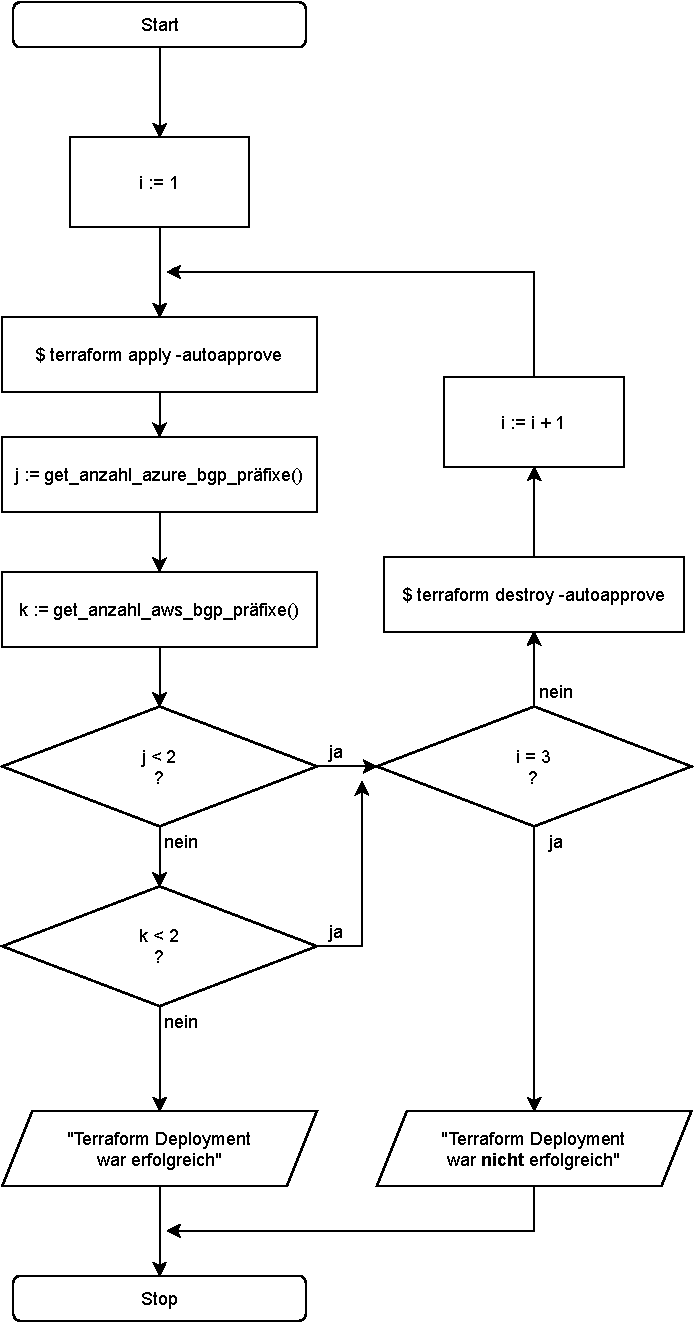
\includegraphics{Figures/programmablaufplan_bash_deploy_tf.pdf}
  \caption{TF Redeployment Bash Skript}
  \label{grafik:programmablaufplan_bash_deploy_tf}
\end{figure}\FloatBarrier

%Programmablaufdiagramm

Durch das Bash-Skript wurde dieser Bug nicht zum Showstopper, allerdings hat das Deployment manchmal länger gedauert (Normale Deployment Zeit * Versuche).

%FIX vom https://github.com/hashicorp/terraform-provider-aws/pull/19077
Dieser Bug wurde angeblich noch kurz vor Abgabe dieser Arbeit mit PR\# gefixt, allerdings konnte das nicht mehr getestet werden. Es ist im Commit ersichtlich, dass es sich um einen Bug in der Sortierfunktion handelte.

\textbf{\underline{Zustandslose VyOS-Konfiguration}}\\
%Terraform Einleitung
Terraform speichert, wie bereits erläutert, alle Referenzen auf Infrastrukturkomponenten in der Datei terraform.tfstate. Da es für VyOS keinen vollwertigen Terraform-Provider gibt, wurde mit Templates, die verschiedene set-Kommandos ausführen, gearbeitet. Diese Konfigurationsänderungen sind dadurch völlig zustandlos, da sie nicht invertierbar sind: Terraform kennt nicht die Umkehrung der "set"-Kommandos, welche benötigt würden, um bei einen \glqq terraform destroy\grqq{} die Konfigurationen am VyOS-Router rückgängig zu machen.
%https://www.terraform.io/docs/language/resources/provisioners/syntax.html#destroy-time-provisioners
Ein Ansatz wäre gewesen, ein weiteres Template zur Verfügung zu stellen, in dem alle set- durch delete-Kommandos negiert werden.\\
\begin{lstlisting}[label=set-delete-vyos,caption=delete negiert das vorherige set-Kommando.]
vyos@vyos-cloud# set system time-zone Europe/Berlin
[edit]
vyos@vyos-cloud# delete system time-zone Europe/Berlin
[edit]
\end{lstlisting}
Per \textit{Destroy-Time Provisioner} würde dieses Template nur bei einem \textit{terraform destroy} genutzt werden. Das Problem ist, dass schon bei minimalen Änderungen des Deploy-Templates auch das Destroy-Template angepasst werden muss. Weiterhin sind die IPSEC-Konfigurationen relativ umfangreich. Es war zu befürchten, dass Relikte aus der Konfiguration übrig bleiben, wenn die Negation aus unbekannten Gründen fehlschlug.

Eine weitere Idee war, mit dem VyOS-Feature "rollback" zu arbeiten. Über eine commit-History werden alle Änderungen an dem System dokumentiert.
\begin{lstlisting}[label=commit-history-vyos,caption=Commit History VyOS]
vyos@vyos-cloud:~$ show system commit | head -3
0   2021-05-05 09:47:51 by tf via cli
1   2021-05-05 09:25:24 by tf via other
2   2021-05-04 21:17:57 by vyos via cli
\end{lstlisting}

So würde man die letzte Revision \textit{vor} der Konfiguration der Backbone-Verbindungen festhalten, um bei einem \textit{terraform destroy} darauf zurückgehen zu können.

\begin{lstlisting}[label=rollback-cmd-vyos,caption=Rollback auf Revision N nach Reboot]
vyos@vyos-cloud# rollback
Possible completions:
  <N>   Rollback to revision N (currently requires reboot)

  Revisions:
    0   2021-05-05 09:47:51 tf by cli
    1   2021-05-05 09:25:24 tf by other
    2   2021-05-04 21:17:57 vyos by cli
\end{lstlisting}

Es wurden zwei Bash-Skripte geschrieben: \textit{save\_last\_manual\_commit.sh} speichert die letzte Revision lokal auf dem VyOS-Router, \textit{apply\_last\_manual\_commit.sh} macht einen Rollback.

\begin{lstlisting}[label=save-last-commit-vyos,caption=Bla]
resource "null_resource" "vyos_config" {
  connection {
    type = "ssh"
    host = var.vyos_host
    user = var.ssh_user
    private_key = file(var.private_key_file)
  }
  [...]
  provisioner "local-exec" {
    command = "${path.module}/bin/save_last_manual_commit.sh"
  }
}
\end{lstlisting}

Nach \textit{terraform apply} liegt auf dem VyOS-Router eine Datei, die den letzten Timestamp der letzten \glqq händischen\grqq{} festhält.

\begin{lstlisting}[label=save-last-commit-file-vyos,caption=Blub]
vyos@vyos-cloud# cat ~tf/last_manual_commit.txt
2021-05-05 09:47:51 by tf via cli
\end{lstlisting}

Bei \textit{terraform destroy} wird das Skript \textit{apply\_last\_manual\_commit.sh} via Terraform \textit{Destroy-Time Provisioner} ausgeführt, welches den Rollback hin zu dem gespeicherten Zeitpunkt auf dem VyOS Router veranlasst.

\begin{lstlisting}[label=apply-last-commit-vyos,caption=Blub]
resource "null_resource" "vyos_config_destroy" {
  provisioner "local-exec" {
    when = destroy
    command = "${path.module}/bin/apply_last_manual_commit.sh"
  }
}
\end{lstlisting}

\textbf{\underline{Lange Laufzeiten für Erstellung von Azure VPN Gateway}}\\
%https://docs.microsoft.com/en-us/azure/vpn-gateway/vpn-gateway-about-vpngateways#whatis
Die Erstellung des Azure VPN Gateways kann bis zu 45 Minuten in Anspruch nehmen. In der Praxis waren es meist ~25 Minuten für den Standort "North Europe". Auch das Löschen eines VPN Gateways via \textit{terraform destroy} dauerte bis zu 15 Minuten. Nur wenn dieses Gateway gelöscht wurde, kann ein \textit{Re-Deploy} erfolgen, welches vor allem dann notwendig ist, wenn die Vertauschung von IPSEC-Parametern (s.o.) eintrifft.\\
Bei diesem Phänomen handelt es sich nicht um einen Bug im eigentlichen Sinne, macht aber das Deployment z.B. für Live-Demonstrationen nicht praktikabel. Da alle weiteren Use-Cases auf diesem Use-Case 1 aufbauen und ebenso in Terraform abgebildet werden sollten, musste eine Lösung gefunden werden, um die Deployment-Zeiten zu verkürzen, da jede Änderung des Codes ein (teilweises) Re-Deployment notwendig macht (vgl. später).

%Dies wird zum Beispiel gebraucht, wenn an der Konfiguration der Infrastruktur Änderungen vorgenommen werden, da Terraform durch diese State-Datei weiß, dass 

\iffalse
%Deadlock? Race Condition?
\textbf{\underline{Deadlock Site-2-Site-Verbindung AWS <-> Azure}}
%Fakeconnection erzeugen

Beim Testen der ersten geschriebenen Terraform-Module kam es zu einer Deadlock-Situation, bei der das \glqq terraform apply\grqq{}-Kommando in einen Timeout lief.
\begin{lstlisting}[label=timeout_aws_azure_ip_deadlock,caption=Deadlock AWS <-> Azure.]
BLA
\end{lstlisting}

%Abgrenzung: alle Public-IP und Private-IP beziehen sich auf IPv3!!!
Bei genauerer Untersuchung stellte sich heraus, dass kein Bug in Terraform vorlag, vielmehr hatte sich ein Logikbug eingeschlichen. Azure erzeugt standardmäßig die Public-IP-Adresse für das Azure-eigene VPN Gateway erst, sobald die \textit{erste VPN-Gegenstelle} konfiguriert wurde. Für die Konfiguration muss allerdings die Public-IP der jeweiligen Gegenstelle angegeben werden. Das Virtual private gateway von AWS legt eine Public-IPv4-Adresse pro Gegenstelle an: 

Dieses Problem ist nicht Terraform geschuldet, sondern eher der Logik, wie die VPN-Verbindungen in Azure bzw. AWS konfiguriert werden 
Dieses Problem tritt in dieser Form nicht mit Verbindungen mit dem Private Cloud-Router auf, da die Public IP-Adresse bereits vor der Ausführung von Terraform bekannt ist.
Fake Gegenstelle...
\fi
\subsection{Evaluation}
Nach dem erfolgreichen Deployment wird folgender Status von Terraform zurückgemeldet. Die letzte Zeile stammt vom Deploy-Skript:
\begin{lstlisting}[label=tf-base-deployment-ok,caption=Terraform Deployment Status]
Apply complete! Resources: 29 added, 0 changed, 0 destroyed.

Outputs:

aws_subnet_id = "subnet-0192ae38a3a16f584"
[... weitere Output-Variablen ...]
\end{lstlisting}

Die im IPAM reservierten Netze sind in AWS als Subnets wiederzufinden. Die Prüfung analog für Azure ist ebenso erfolgreich.

%AWS Screenshot
%IPAM Screenshot


\begin{lstlisting}[label=tf-base-deployment-ipsec-ok,caption=IPSEC Status]
vyos@vyos-cloud:~$ show vpn ipsec sa
Connection                     State    Uptime
-----------------------------  -------  --------
[...]
peer-20.67.209.254-tunnel-vti  up       4h43m19s [...]
peer-3.65.181.187-tunnel-vti   up       4h47m26s [...]
\end{lstlisting}

Die Adressen gehören dabei zu Amazon bzw. Microsoft.

\begin{lstlisting}[label=whois-amazon-public-ip,caption=Diese Adresse gehört Amazon. Analog wurde geprüft für 20.67.209.254 (Microsoft).]
$ whois 3.65.181.187 | grep -A2 NetRange
NetRange:       3.64.0.0 - 3.79.255.255
CIDR:           3.64.0.0/12
NetName:        AMAZON-FRA
\end{lstlisting}

Außerdem wurden auf dem Cloud-Router die AWS- und Azure-Präfixe via BGP installiert. Pro Präfix sind zwei Pfade vorhanden (s.o.).
...s. Listing xy in Lösungsfindung...

Es wurde pro Cloud eine virtuelle Maschine (Ubuntu) installiert, um die Ende-zu-Ende-Konnektivität zu prüfen. Dieser Ping von AWS VPC -> Azure VNET war erfolgreich. Analog waren alle weiteren Ping-Tests zwischen den Cloud-Plattformen erfolgreich:

\begin{lstlisting}[label=tf-base-deployment-ping-ok,caption=Ping Tests zwischen verschiedenen Cloud-Plattformen]
ubuntu@ip-10-33-0-121:~$ ping -c1 10.32.0.4
PING 10.32.0.4 (10.32.0.4) 56(84) bytes of data.
64 bytes from 10.32.0.4: icmp_seq=1 ttl=63 time=25.7 ms

--- 10.32.0.4 ping statistics ---
1 packets transmitted, 1 received, 0% packet loss, time 0ms
rtt min/avg/max/mdev = 25.729/25.729/25.729/0.000 ms
\end{lstlisting}

Es wurden vereinzelte Messungen in verschiedene Richtungen mit dem Tool \textsf{iperf3} gemacht, die grundsätzlich \glqq ordentliche\grqq{} Bandbreiten versprechen, so bspw.:

%Messung Sender vyos-aws -> vyos-azure
\begin{minted}[breaklines,frame=single]{bash}
root@vyos-aws-ovpn-gw:~# iperf3 -c 10.32.0.5
Connecting to host 10.32.0.5, port 5201
[  4] local 10.33.2.93 port 44298 connected to 10.32.0.5 port 5201
[ ID] Interval           Transfer     Bandwidth       Retr  Cwnd
[  4]   0.00-1.00   sec  32.8 MBytes   275 Mbits/sec   45   1.52 MBytes
[  4]   1.00-2.00   sec  41.2 MBytes   346 Mbits/sec    0   1.66 MBytes
[  4]   2.00-3.00   sec  40.0 MBytes   336 Mbits/sec    0   1.78 MBytes
[  4]   3.00-4.00   sec  37.5 MBytes   315 Mbits/sec   17   1.33 MBytes
[  4]   4.00-5.00   sec  33.8 MBytes   283 Mbits/sec    0   1.40 MBytes
[  4]   5.00-6.00   sec  41.2 MBytes   346 Mbits/sec    0   1.45 MBytes
[  4]   6.00-7.00   sec  41.2 MBytes   346 Mbits/sec    0   1.49 MBytes
[  4]   7.00-8.00   sec  43.8 MBytes   367 Mbits/sec    0   1.51 MBytes
[  4]   8.00-9.00   sec  42.5 MBytes   357 Mbits/sec    0   1.52 MBytes
[  4]   9.00-10.00  sec  41.2 MBytes   346 Mbits/sec    0   1.53 MBytes
- - - - - - - - - - - - - - - - - - - - - - - - -
[ ID] Interval           Transfer     Bandwidth       Retr
[  4]   0.00-10.00  sec   395 MBytes   332 Mbits/sec   62             sender
[  4]   0.00-10.00  sec   394 MBytes   330 Mbits/sec                  receiver
\end{minted}

Man sieht allerdings an der vorletzten Zeile (\glqq Retr 62\grqq{}), dass TCP Retransmissions stattgefunden haben. Es ist wahrscheinlich, dass ein \textit{Bottleneck} existiert, Paketverluste konnten mit diversen Ping-Messungen (s.o.) nicht festgestellt werden. Wie in der Abgrenzung geschrieben, werden Bandbreiten, insofern sich nicht ein deutlicher negativer \textit{Impact} bemerkbar macht, in dieser Arbeit nicht tiefergehend untersucht, s. Ausblick...

Floodping:
\begin{minted}[breaklines,frame=single]{bash}
root@vyos-azure-ovpn-gw:~# /bin/ping -s 1200 -c 1000 -f 10.33.2.93
PING 10.33.2.93 (10.33.2.93) 1200(1228) bytes of data.

--- 10.33.2.93 ping statistics ---
1000 packets transmitted, 1000 received, 0% packet loss, time 13370ms
rtt min/avg/max/mdev = 25.968/28.533/173.755/10.763 ms, pipe 11, ipg/ewma 13.384/27.159 ms
\end{minted}
\fi


%Härtung IPSEC Parameter? GCM usw...
%BFD für schneller Konvergenzzeiten? -> Ausblick...
%RTT und Ping in Einleitung / ICMP

Es wurden außerdem in von allen Teilnehmern zu allen Teilnehmern Ping-Tests gemacht und währenddessen eine Verbindung getrennt. Da ein Präfix über zwei Pfade zu sehen ist, ist die Erwartung, dass ein Backup-Pfad genutzt wird. Man kann an folgendem Beispiel sehr gut erkennen, dass das BGP eine Konvergenzzeit erfordert, bis die Pakete über einen anderen Pfad laufen. \textit{ping} versendet in der Standardkonfiguration im Interval von einer Sekunde ICMP-Echo-Pakete. Daraus lässt sich schlussfolgern, dass die Verbindung im unteren Beispiel etwa 44 Sekunden unterbrochen war.\\
Weiterhin hat sich die Round-Trip-Time von ~20 ms auf ~62 ms erhöhtt. Dies ist eine logische Konsequenz, da Pakete nun längere Wege zurücklegen müssen. Alle Ping-Tests waren trotz Kappen einer Verbindung erfolgreich. Man muss dabei allerdings Paketverluste während der Konvergenzzeit hinnehmen.
%Typische BGP Konvergenzzeiten?

\begin{figure}[h]
  \centering
  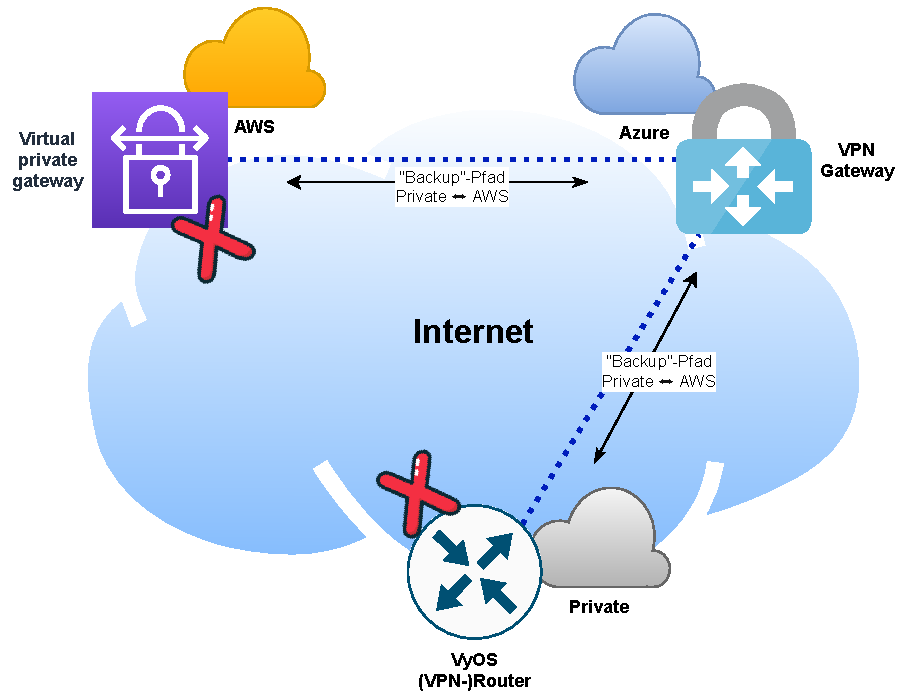
\includegraphics{Figures/Use-Case-1_Basis_Deployment_missing_link.pdf}
  \caption{TF Deployment with missing link}
  \label{grafik:Use-Case-1_Basis_Deployment_missing_link}
\end{figure}

\begin{lstlisting}[label=tf-base-deployment-ping-ok,caption=Ping Tests zwischen verschiedenen Cloud-Plattformen mit Kappen einer Backbone-Verbindung.]
root@www:~# ping 10.33.0.121
PING 10.33.0.121 (10.33.0.121) 56(84) bytes of data.
[...]
64 bytes from 10.33.0.121: icmp_seq=15 ttl=61 time=19.9 ms
64 bytes from 10.33.0.121: icmp_seq=16 ttl=61 time=24.3 ms
64 bytes from 10.33.0.121: icmp_seq=17 ttl=61 time=19.6 ms
64 bytes from 10.33.0.121: icmp_seq=18 ttl=61 time=19.7 ms <-- Kappen einer Verbindung
64 bytes from 10.33.0.121: icmp_seq=62 ttl=61 time=67.4 ms <-- Revovery ueber Backup-Pfad
64 bytes from 10.33.0.121: icmp_seq=63 ttl=61 time=62.2 ms
64 bytes from 10.33.0.121: icmp_seq=64 ttl=61 time=62.5 ms
64 bytes from 10.33.0.121: icmp_seq=65 ttl=61 time=62.4 ms
[...]
\end{lstlisting}

